\chapter{Next Steps and Moving to 2D\label{ch:5_2DGKP}}


In the previous chapter, we presented the results of our experiments with a fluxonium in a 3D cavity. We demonstrated a tunable dispersive shift between the qubit and the storage resonator via bosonic mode threading and characterized the various components of our system. In doing so, we discovered that the lifetime of the storage mode was \textit{significantly} lower than expected (as compared to its bare value) whenever the qubit chip was inserted into the resonator package. After many rounds of experimentation and testing, we were ultimately able to attribute this effect to two main sources: (i) the storage mode's coupling to the lossy qubit flux line; and (ii), its participation in spurious slotline modes of the 3D superconducting package. While the former issue could in principle be solved via clever microwave engineering and filtering, the latter unfortunately is intrinsic to our 3D design and not easily remedied. As we came to learn, it is generally difficult to integrate fast-flux into a 3D cavity while also maintaining the cavity coherence. 

There are certain approaches that have been proposed and implemented in the literature that work towards integrating fast-flux in 3D. One such example is the magnetic hose from Refs. \cite{gargiulo2021fast,valadares2023demand}. Here, the authors route flux from an external coil to a tunable transmon qubit in a 3D superconducting package using a ``hose'' composed of concentric aluminium and mu-metal layers. In the experiment of Ref. \cite{valadares2023demand} specifically, this is done for the purpose of bosonic cQED, and the authors demonstrate that the lifetime of their 3D storage resonator is not limited by their flux delivery mechanism. Unfortunately, however, the design and implementation of a magnetic hose is quite painstaking, and would require a full redesign of both the cavities and the fluxonium chips that were presented in Ch. \ref{ch:4_3DGKP}. Other designs have also been proposed recently, e.g. Ref. \cite{hutin2024monitoring} or Ref. \cite{maiti2024ancilla}, which both rely on some form of on-chip distributed-element microwave filtering to prevent losses from the flux line at the frequency of the storage. Despite requiring more advanced microwave engineering in design, these approach seem promising for integrating fast-flux in 3D while maintaining the storage resonator lifetime. 

In our case, however, after discovering the root cause of our storage coherence issues and identifying various avenues to proceed from there, we decided to forgo the 3D architecture entirely. This was in part due to the time and difficulty of implementing fast-flux delivery in 3D (which, as highlighted above, is a difficult project in of itself); but it was also a choice we made consciously, motivated by the idea of moving our experiments to 2D. Over the course of our 3D-GKP project, we ended up developing an entirely separate but novel way to do GKP error correction in 2D, using a microwave-activated coupler to generate faster conditional displacements. This 2D project, first proposed using a transmon control qubit and later a fluxonium, represents an improvement over the ``direct dispersive'' approach we took in our 3D-GKP project in most ways. As such, we decided that moving to 2D is a more promising long term path towards building extensible GKP error correction systems. 

In this chapter, we present three of our proposals for implementing GKP error correction in 2D. Within our bosonic subgroup in EQuS, we refer to these as the ``RAT'' (see Ch. \ref{sec:5_RAT}), the ``RAF'' (see Ch. \ref{sec:5_RAF}), and the ``2D dispersive'' (see Ch. \ref{sec:5_2D_Disp}) approaches, respectively\footnote{The meaning behind these names will become apparent shortly!}. We will go through the basic theory for all three approaches and discuss high-level results: in particular, we have already completed designs for the RAF and 2D dispersive projects, which are currently being fabricated as of this writing. 

Here, my aim is give a broad overview to our upcoming 2D experiments; however, more details and a discussion of the careful design and simulation considerations taken can be found in the SM thesis of Shantanu Jha. 
\clearpage


\section{The Asymmetrically-Threaded-SQUID Coupler \label{sec:5_RAT}}

The core insight that motivated our investigation into GKP error correction in 2D was that we can use an Asymmetrically-Threaded SQUID (ATS) as a coupler element to realize the desired ``three-wave mixing'' conditional displacement term that underpins all GKP QEC schemes. The ATS is a superconducting dipole element consisting of a symmetric SQUID shunted by an inductor, as shown in Fig. \ref{fig:5_ats_spectrum}(a); the two resulting flux loops in the circuit are then typically biased \textit{asymmetrically} \cite{lescanne2020exponential, berdou2023one}. In practice, the inductor is realized using an array of Josephson junctions and so the circuit itself is similar to that of a gradiometric SNAIL \cite{miano2022frequency}; it was also recently referred to as the Linear Inductive Coupler when biased symmetrically \cite{maiti2024ancilla}. Despite these various names, we will refer to the actual dipole element as an ATS throughout our work, irrespective of its bias point. 

\begin{figure}[h]
    \centering
    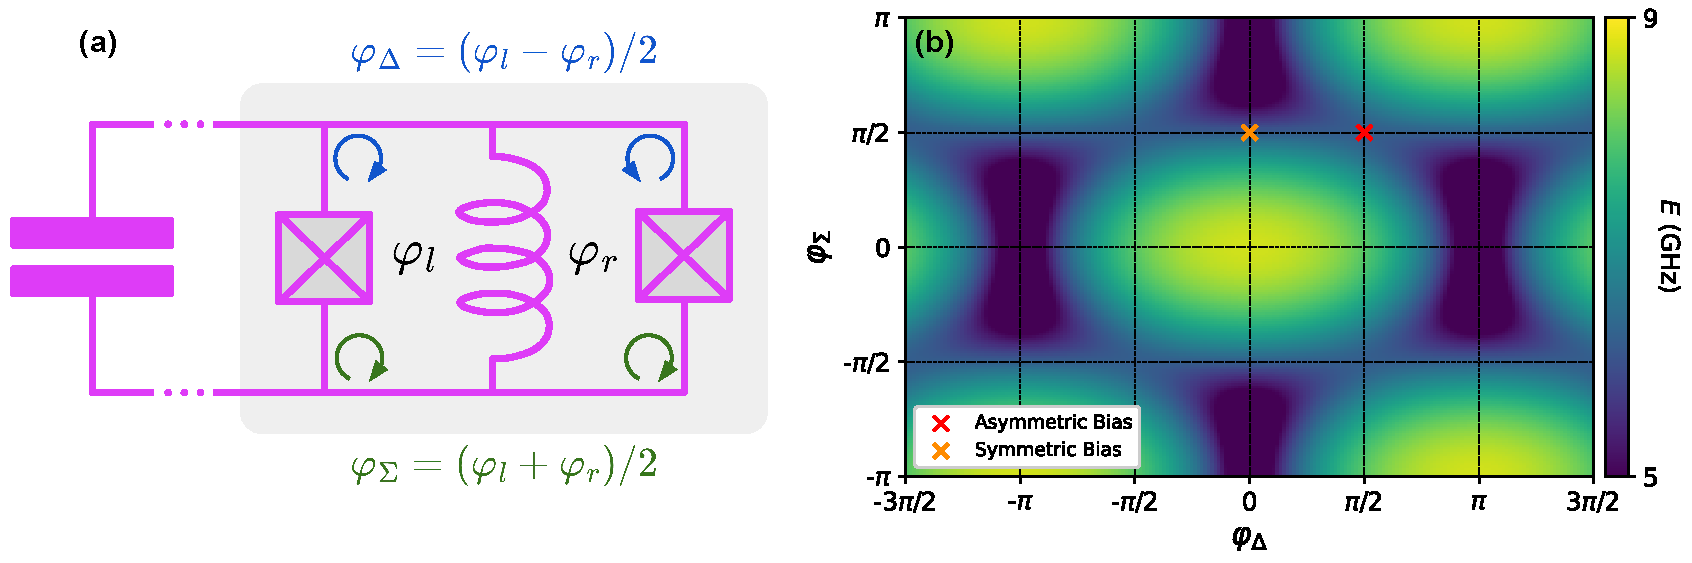
\includegraphics[width=\linewidth]{Figures/5/ats_spectrum.pdf}
    \caption{\textbf{(a)} Circuit diagram for the ATS dipole element (shaded in gray) which consists of a symmetric SQUID shunted by an inductor. The left/right loops are threaded by fluxes $\varphi_l$/$\varphi_r$ respectively, giving rise to common and differential fluxes $\varphi_\Sigma$ and $\varphi_\Delta$. When the ATS is connected to a capacitor, it forms a mode. \textbf{(b)} Fundamental frequency of the ATS mode vs. flux $(\varphi_\Sigma, \varphi_\Delta)$ using parameters $E_L/h = 60$ GHz, $E_J/h = 30$ GHz, and $E_C/h = 80$ MHz.}
    \label{fig:5_ats_spectrum}
\end{figure}

\noindent To begin our exploration of the ATS, let's consider its potential energy, which is given by:
\begin{equation}
    \hat{U}_b = \frac{1}{2}E_L \bigg(\hat{\varphi} + \frac{C_r\varphi_r - C_l\varphi_l}{C_\Sigma}\bigg)^2 - E_{J,l}\cos\!\bigg(\hat{\varphi} + \frac{C_r}{C_\Sigma}[\varphi_l + \varphi_r]\bigg) - E_{J,r}\cos\!\bigg(\hat{\varphi} - \frac{C_l}{C_\Sigma}[\varphi_l + \varphi_r]\bigg)
\end{equation}
Here, we have used the method of Ref. \cite{you2019circuit} to write the potential in terms of its irrotational variable $\hat{\varphi}$, which is the correct approach for time-varying external fluxes; the expression is thus somewhat different from the original description of the ATS in Ref. \cite{lescanne2020exponential}. We have left and right junctions with energies $E_{J, l/r}$, inherent capacitances $C_{l/r}$, and external fluxes $\varphi_{l/r}$ respectively. At this point, we can define the effective $E_J = (E_{J,l} + E_{J,r})/2$ and asymmetry $\Delta E_J = (E_{J,l} - E_{J,r})/2$, and transform to sum and difference coordinates $\varphi_{\Sigma/\Delta} = (\varphi_l \pm \varphi_r)/2$.  Ideally, we would like the junctions to be perfectly symmetric; in practice the asymmetry can be minimized to about $1\%$ of $E_J$. While this is important to keep track of, we will here set $\Delta E_J \to 0$ in the rest of the theory that follows. Thus, $E_{J,l} = E_{J,r} = E_J$ and $C_l = C_r = C$, with $C_\Sigma = C_l + C_r$. We can therefore simplify the complicated expression above and write the potential as:
\begin{equation}
\hat{U}_b(\hat{\varphi}) = \frac{1}{2}E_L(\hat{\varphi} - \varphi_\Delta)^2 - 2E_J \cos(\varphi_\Sigma)\cos(\hat{\varphi})
\end{equation}
In what follows, we will typically keep the differential flux $\varphi_\Delta$ constant and only modulate the common flux $\varphi_\Sigma = \varphi_\Sigma(t)$. Therefore, we can perform a gauge transformation to move the now DC flux $\varphi_\Delta$ to the cosine via $\hat{\varphi} \mapsto \hat{\varphi} + \varphi_\Delta$. This finally get us back to the familiar expression
\begin{equation}
\hat{U}_b(\hat{\varphi}) = \frac{1}{2}E_L\hat{\varphi}^2 - 2E_J \cos(\varphi_\Sigma)\cos(\hat{\varphi} + \varphi_\Delta)
\end{equation}
that can be found in Refs. \cite{lescanne2020exponential, berdou2023one}. We will use this throughout the rest of this chapter.

As shown in Fig. \ref{fig:5_ats_spectrum}(b), when the ATS is connected to a capacitance, the resulting mode has a fundamental frequency that is doubly periodic in $\varphi_\Sigma$ and $\varphi_\Delta$, forming an `egg-carton' potential as it is sometimes referred to. There are two typical operating points for the ATS:

\begin{itemize}
    \item \textbf{Asymmetric bias point:} $(\varphi_\Sigma, \varphi_\Delta) = (\pi/2, \pi/2)$, corresponding to $\varphi_l = \pi$ and $\varphi_r = 0$. This is the standard operating point for the ATS. By modulating the sum flux around this bias, i.e. $\varphi_\Sigma(t) = \pi/2 + \epsilon(t)$, we get the following time-dependent potential for the ATS dipole:
    \begin{equation}
        \hat{U}_b(\hat{\varphi}) = \frac{1}{2}E_L \hat{\varphi}^2 - 2E_J \sin[\epsilon(t)]\sin(\hat{\varphi})
    \end{equation}
\item \textbf{Symmetric bias point:} $(\varphi_\Sigma, \varphi_\Delta) = (\pi/2, 0)$, corresponding to $\varphi_l = \varphi_r = \pi/2$. Biasing here gives us:
\begin{equation}
        \hat{U}_b(\hat{\varphi}) = \frac{1}{2}E_L \hat{\varphi}^2 - 2E_J \sin[\epsilon(t)]\cos(\hat{\varphi})
    \end{equation}
\end{itemize}
%%%%%%%%%%%%%%%%%%%%%%%%
\subsection{The Resonator-ATS-Transmon (RAT)}

Our first approach to faster GKP error correction was developed using the ATS as a coupler element between a storage resonator and a transmon control qubit. We name this the RAT. The basic idea relies on black-box quantization (cf. Ch. \ref{ch:3_cQED}) between the three modes $\hat{a}_0$, $\hat{b}_0$, and $\hat{q}_0$ for the resonator, ATS, and transmon respectively. The bare transmon Hamiltonian is:
\begin{equation}
\hat{H}_{q, 0} = 4E_{C,q}\hat{n}_q^2 - E_{J,q}\cos(\hat{\theta}) = \omega_{q,0}\,\hat{q}_0^\dagger \hat{q}_0 - \Big[E_{J,q}\cos(\hat{\theta}) + \frac{1}{2}E_{J,q} \hat{\theta}^2\Big] 
\end{equation}
where we write the mode $\hat{q}_0$ in terms of the transmon charge $\hat{n}_q$ and phase-drop $\hat{\theta}$. For the ATS, it is:
\begin{equation}
\hat{H}_{b,0} = 4E_C \hat{n}^2 + \hat{U}_b(\hat{\varphi}) = \omega_{b,0}\hat{b}_0^\dagger \hat{b}_0 - 2E_J \cos(\varphi_\Sigma)\cos(\hat{\varphi} + \varphi_\Delta)
\end{equation}
in terms of the ATS charge operator $\hat{n}$ and phase-drop $\hat{\varphi}$. Finally, for the storage we have $\hat{H}_{a, 0} = \omega_{a,0}\hat{a}_0^\dagger \hat{a}_0$. If we take the modes to be linearly coupled (e.g. via capacitive coupling) in series, i.e. resonator $\leftrightarrow$ ATS $\leftrightarrow$ transmon, then the total Hamiltonian has a \textit{linear} part:
\begin{equation}
\hat{H}_{\rm lin, 0} = \omega_{a,0}\hat{a}_0^\dagger \hat{a}_0 + \omega_{b,0}\hat{b}_0^\dagger \hat{b}_0 + \omega_{q,0}\hat{q}_0^\dagger \hat{q}_0 - g_{ab}(\hat{a}_0 - \hat{a}_0^\dagger)(\hat{b}_0 - \hat{b}_0^\dagger) - g_{qb}(\hat{b}_0 - \hat{b}_0^\dagger)(\hat{q}_0 - \hat{q}_0^\dagger)
\end{equation}
Following black-box quantization, we can diagonalize $\hat{H}_{\rm lin, 0}$ as a system of normal modes $\hat{a}$ (storage-like), $\hat{b}$ (buffer-like), and $\hat{q}$ (qubit-like). In this basis $\hat{H}_{\rm lin} = \omega_a \hat{a}^\dagger\hat{a} + \omega_b \hat{b}^\dagger\hat{b} + \omega_q \hat{q}^\dagger\hat{q}$, where $\omega_a$, $\omega_b$, and $\omega_q$ are the normal mode frequencies. We can also rewrite the bare modes in this normal mode basis via a linear transformation:
\begin{align}
\hat{\theta} &= \theta_{q, 0}(\hat{q}_0 + \hat{q}_0^\dagger) = \theta_q(\hat{q} + \hat{q}^\dagger) + \theta_b(\hat{b} + \hat{b}^\dagger) + \theta_a(\hat{a} + \hat{a}^\dagger) \\
\hat{\varphi} &= \phi_{b, 0}(\hat{b}_0 + \hat{b}_0^\dagger) = \phi_q(\hat{q} + \hat{q}^\dagger) + \phi_b(\hat{b} + \hat{b}^\dagger) + \phi_a(\hat{a} + \hat{a}^\dagger)
\end{align}
Here, $\theta_i$ denotes the participation of mode $i$ in the phase across the Josephson junction in the transmon, while $\phi_i$ is the participation in the phase across the ATS. In total, we have
\begin{equation}
\hat{H} = \sum_{c = \{a, b, q\}}\omega_c \hat{c}^\dagger\hat{c} - \Big[E_{J,q}\cos(\hat{\theta}) + \frac{1}{2}E_{J,q} \hat{\theta}^2\Big] - 2E_J \cos(\varphi_\Sigma)\cos(\hat{\varphi} + \varphi_\Delta)
\end{equation}
as the Hamiltonian for the full resonator-ATS-transmon system written in the ``black-box quantization'' basis (i.e. of the normal modes of the linearized circuit). 

With the Hamiltonian written down, let's now see how to get conditional displacements out of it. We park the ATS at its standard asymmetric bias point $(\varphi_\Sigma, \varphi_\Delta) = (\pi/2, \pi/2)$ and modulate $\varphi_\Sigma(t) = \pi/2 + \epsilon(t)$ about this. The ATS potential takes on the form $\sin[\epsilon(t)]\sin(\hat{\varphi})$, and so we can Taylor expand $\sin[\epsilon(t)] \approx \epsilon(t)$ and $\sin(\hat{\varphi}) \approx \hat{\varphi} - \hat{\varphi}^3/6$ in anticipation of making a rotating-wave approximation. We can also truncate the transmon potential to a Duffing oscillator, considering only the leading fourth-order nonlinearity. These approximations give us
\begin{equation}
\hat{H} = \sum_{c = \{a, b, q\}}\omega_c \hat{c}^\dagger\hat{c} - \frac{E_{J,q}}{24}\hat{\theta}^4 - 2E_J \epsilon(t)\hat{\varphi} + \frac{1}{3}E_J\epsilon(t)\hat{\varphi}^3
\end{equation}
We go into a rotating frame for each of the modes $\hat{c} \mapsto \hat{c} e^{-i\tilde{\omega}_c t}$ where we set the frequency $\widetilde{\omega}_c = \omega_c - \theta_{c}^{2} \big[\theta_{a}^{2} + \theta_{b}^{2} + \theta_{q}^{2}\big]/2$ to cancel out the frequency normalizations that arise from the transmon nonlinearity. In this frame, we get
\begin{align}
\begin{split}
\hat{H} &= \hat{H}_{cc} - \frac{E_{J,q}}{24}\Big[\theta_q(\hat{q}e^{-i\tilde{\omega}_q t} + \hat{q}^\dagger e^{i\tilde{\omega}_q t}) + \theta_b(\hat{b}e^{-i\tilde{\omega}_b t} + \hat{b}^\dagger e^{i\tilde{\omega}_b t}) + \theta_a(\hat{a}e^{-i\tilde{\omega}_a t} + \hat{a}^\dagger e^{i\tilde{\omega}_a t})\Big]^4 \\&\quad- 2E_J\epsilon(t)\Big[\phi_q(\hat{q}e^{-i\tilde{\omega}_q t} + \hat{q}^\dagger e^{i\tilde{\omega}_q t}) + \phi_b(\hat{b}e^{-i\tilde{\omega}_b t} + \hat{b}^\dagger e^{i\tilde{\omega}_b t}) + \phi_a(\hat{a}e^{-i\tilde{\omega}_a t} + \hat{a}^\dagger e^{i\tilde{\omega}_a t})\Big]\\ &\quad + \frac{1}{3}E_J\epsilon(t)\Big[\phi_q(\hat{q}e^{-i\tilde{\omega}_q t} + \hat{q}^\dagger e^{i\tilde{\omega}_q t}) + \phi_b(\hat{b}e^{-i\tilde{\omega}_b t} + \hat{b}^\dagger e^{i\tilde{\omega}_b t}) + \phi_a(\hat{a}e^{-i\tilde{\omega}_a t} + \hat{a}^\dagger e^{i\tilde{\omega}_a t})\Big]^3
\end{split}
\end{align}
where $\hat{H}_{cc} = \sum (\omega_c - \tilde{\omega}_c)\hat{c}^\dagger\hat{c}$ will cancel out when the terms are expanded. At this point our task involves sorting through the various pumped nonlinear terms and keeping only the ones that survive the RWA. We set $\epsilon(t) = \epsilon_p \sin(\omega_p t)$ with $\omega_p = \tilde{\omega}_a$, picking out terms that rotate at the (renormalized) storage frequency. Luckily we can do the oscillator expansion, normal ordering, and RWA all numerically using SymPy. The final effective Hamiltonian
\begin{align}
\begin{split}
\hat{H}_{\rm eff} &= \frac{K_a}{2}{{a}^\dagger}^{2} {a}^{2} + \frac{K_b}{2}{{b}^\dagger}^{2} {b}^{2} + \frac{K_q}{2}{{q}^\dagger}^{2} {q}^{2} + \frac{\chi_{ab}}{2}\hat{a}^\dagger\hat{a}\hat{b}^\dagger\hat{b} + \frac{\chi_{aq}}{2} \hat{a}^\dagger\hat{a}\hat{q}^\dagger\hat{q} + \frac{\chi_{qb}}{2} \hat{q}^\dagger\hat{q}\hat{b}^\dagger\hat{b} \\
&\quad + g_{\rm CD}{{q}^\dagger} {q}\big(\hat{a} + \hat{a}^\dagger\big) + g_{\rm disp} \big(\hat{a}+\hat{a}^\dagger\big) + g_a\big[{{a}^\dagger} {a}^{2} + {{a}^\dagger}^{2} {a}\big] + g_b {{b}^\dagger} {b}\big(\hat{a} + \hat{a}^\dagger\big) 
\end{split}
\end{align}
has many terms that we can categorize as follows. We have Kerr nonlinearities for all three modes $K_x = -E_{J, q}\theta_{x}^{4} / 2$ and cross-Kerr dispersive shifts $\chi_{xy} = -2E_{J, q}\theta_{x}^{2} \theta_{y}^{2}$. Next, we have the desired conditional displacement $g_{\rm CD} = E_J\epsilon_{p} \phi_{a} \phi_{q}^{2}$ and an unconditional displacement $g_{\rm disp} = E_J\epsilon_p\big[\phi_a^3 +\phi_{a} \phi_{q}^{2} + \phi_{a} \phi_{b}^{2} - 2\phi_a\big]/2$. Finally, we also have two spurious nonlinear terms associated with the storage and ATS mode: $g_a = E_J\epsilon_{p} \phi_{a}^{3}/2$ and $g_b = E_J\epsilon_{p} \phi_{a}\phi_{b}^{2}$. The qubit anharmonicity $K_q$ should not affect the oscillator dynamics, and just provides the requisite nonlinearity for control. Furthermore, if the ATS is never strongly populated $\ev{\hat{b}^\dagger\hat{b}} \approx 0$, we can further simplify to just:
\begin{equation}
\hat{H}_{\rm eff} = \frac{\chi_{aq}}{2} \hat{a}^\dagger\hat{a}\hat{q}^\dagger\hat{q} + \frac{K_a}{2}{{a}^\dagger}^{2} {a}^{2} + g_{\rm CD}{{q}^\dagger} {q}\big(\hat{a} + \hat{a}^\dagger\big) + g_{\rm disp} \big(\hat{a}+\hat{a}^\dagger\big) + g_a\big[{{a}^\dagger} {a}^{2} + {{a}^\dagger}^{2} {a}\big]
\label{eq:5_FCD_full_hamiltonian}
\end{equation}
Overall, we have the desired conditional displacement term, along with several additional unwanted terms that we will now discuss how to cancel out. Note that all drive-activated terms are proportional to the flux pump envelope $\epsilon_p = \epsilon_p(t)$, which we can pulse to activate the desired interactions. 

\subsection{Conditional Displacements with the RAT}

It turns out that we can cancel many of the unwanted terms above using an echo protocol reminiscent of the echoed conditional displacement (ECD) from Ref. \cite{eickbusch2022fast} that we reviewed in Ch. \ref{ch:2_QEC}. To see how, let's consider a simplified version of Eq. \eqref{eq:5_FCD_full_hamiltonian} with just the CD term and the dispersive shift. We also truncate the transmon to a two-level qubit $\hat{q}^\dagger\hat{q} \to \hat{\sigma}_z$ and thus have:
\begin{equation}
\hat{H}(t) = \frac{\chi}{2}\hat{a}^\dagger\hat{a}[z(t)\hat{\sigma}_z]   + \Big[g_{\rm CD}(t)\hat{a}^\dagger + g_{\rm CD}^\ast(t)\hat{a}\Big]z(t)\hat{\sigma}_z
\label{eq:5_FCD_simplified_hamiltonian}
\end{equation}
Here we have included a fictitious qubit state parameter $z(t) = \ev{\sigma_z(t)}$ that tells us when to perform $\pi$-pulses \cite{eickbusch2022fast}, and also explicitly highlight the time-dependence $g_{\rm CD}(t)$ controlled via the flux pump. We can then solve the Schr\"odinger equation $i\partial_t\hat{U} = \hat{H}(t)\hat{U}$ in terms of a parameterized ansatz $\hat{U}(t)$. We find the same ansatz and solution as Ref. \cite{eickbusch2022fast}: 
\begin{equation}
    \hat{U}(t) = \exp(i\theta \hat{\sigma}_z / 2)\,\exp\!\Big[\hat{a}^\dagger(\gamma + \delta \hat{\sigma}_z) - \hat{a}(\gamma^\ast + \delta^\ast \hat{\sigma}_z)\Big]\exp(i\phi\hat{a}^\dagger\hat{a}\hat{\sigma}_z)
\end{equation}
where $\theta(t), \gamma(t), \delta(t), \phi(t)$ correspond to a qubit rotation, cavity displacement and conditional displacement, and a qubit-selective cavity rotation. Plugging in Eq. \eqref{eq:5_FCD_simplified_hamiltonian} and solving the Schr\"odinger equation, it turns out we can actually find a solution:
\begin{align}
    \begin{split}
        \theta(t) & = +2 \int_0^t d\tau \mathrm{Re}[g_{\rm CD}^*(\tau)\gamma(\tau)] \qquad \qquad\delta(t) = -i \int_0^t d\tau \cos[\phi(\tau)-\phi(t)] g_{\rm CD}(\tau)z(\tau) \\\gamma(t) & = - \int_0^t d\tau \sin[\phi(\tau)-\phi(t)] g_{\rm CD}(\tau)z(\tau) \qquad \qquad\phi(t) = -\frac{\chi}{2} \int_0^t d\tau z(\tau)
    \end{split}
\end{align}
If the CD gate has length $T$, we want $\phi(T) = 0$ at the end of the gate, and thus $\int z(\tau)d\tau = 0$, i.e. the area under the curve of $z(t)$ must be net zero. This implies that the qubit state $z(t)$ has to flip signs at least once! Furthermore, as with the ECD protocol, if we consider only $\pi$-pulses on the qubit, then $z \in \{1, -1\}$. These requirements constrain the pulse schedule $z(t)$ to take on the form of a Walsh function \cite{chalermpusitarak2021frame}. To cancel the \textit{unconditional} displacement and keep just a \textit{conditional} displacement, we next want to set
\begin{equation*}
    \gamma(T) = - \int_0^T \!d\tau \sin[\phi(\tau)] g_{\rm CD}(\tau)z(\tau) = 0, \,\,\text{and}\,\, \delta(T) = -i \int_0^T \!d\tau \cos[\phi(\tau)] g_{\rm CD}(\tau)z(\tau) \neq 0.
\end{equation*}
At this point, observe that if $g_{\rm CD}(t)z(t)$ can be made constant over the gate length $T$, then the symmetries of sine and cosine will automatically ensure $\gamma(T) = 0$ and $\delta(T) \neq 0$. Since the $\pi$-pulse schedule $z(t)$ is constained in its form, we can try several ansatze and modulate $g_{\rm CD}(t)$ with the same time-dependence so that $z(t)g_{\rm CD}(t)$ is constant. We find that a double-echo schedule satisfies all of our requirements, with $\pi$-pulses at $t = T/4$ and $t = 3T/4$, and $z(0)=1$ to initialize the qubit in the ground state $\ket{g}$. An example is plotted below, along with the final pulse sequence for $g_{\rm CD}(t)$ [which, again, is set by modulating the flux pump amplitude $\epsilon_p(t)$]. We named this novel sequence the \textbf{f}ast echoed \textbf{c}onditional \textbf{d}isplacement, or FCD, to contrast it from the usual ``single-echo'' ECD that we saw in Ch. \ref{ch:2_QEC}. 

\begin{figure}[t]
    \centering
    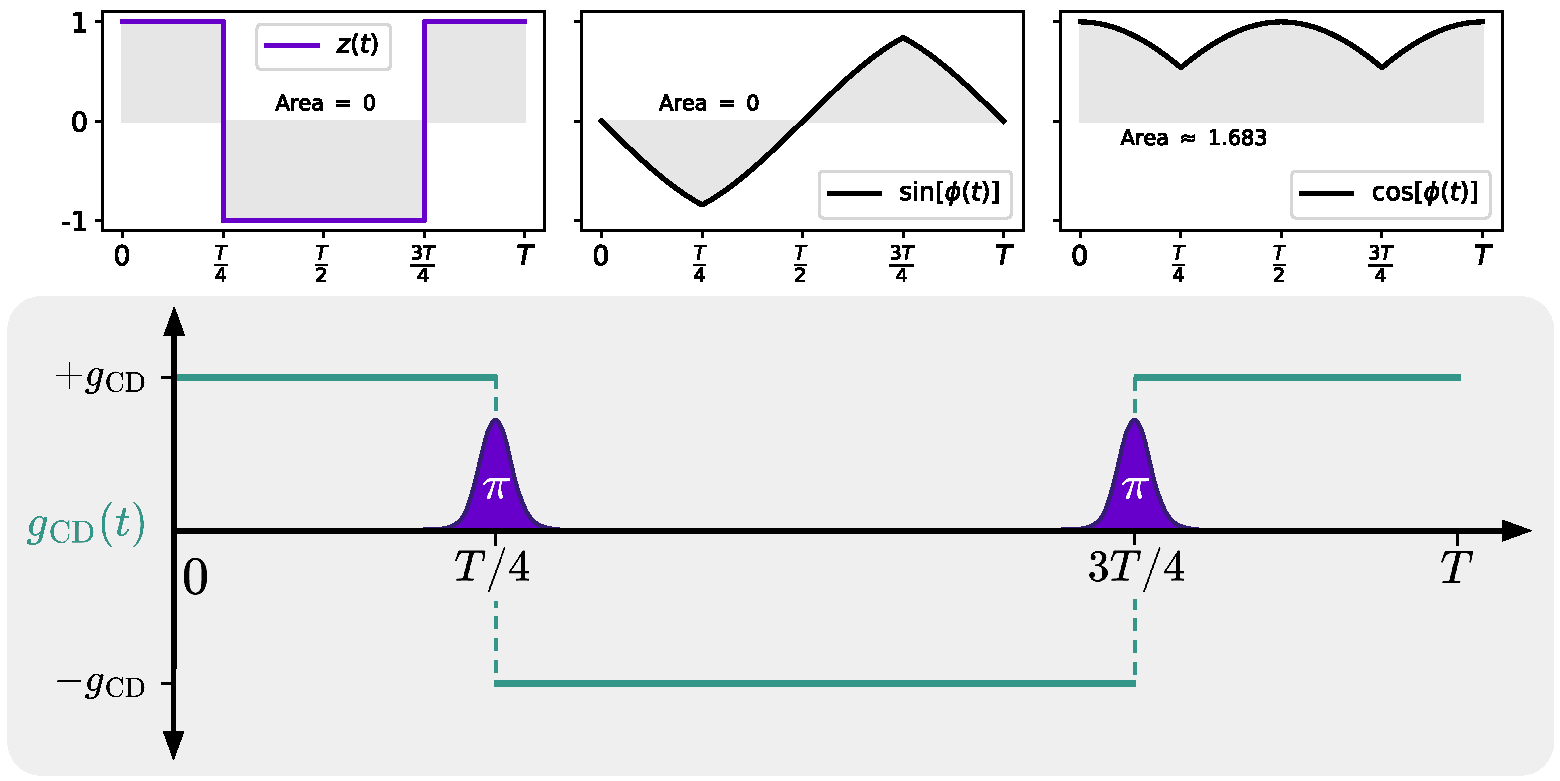
\includegraphics[width=\linewidth]{Figures/5/double_echo_FCD.pdf}
    \caption{FCD pulse implementation using the double-echo $\pi$-pulse schedule $z(t)$. Top row: numerical example of $z(t)$, $\sin[\phi(t)]$, and $\cos[\phi(t)]$ for $T = 2$ and $\chi = 4$. Observe $z(t)$ has an integral of zero as required. By modulating $g_{\rm CD}(t)$ to match the time-dependence of $z(t)$, we get constant $g_{\rm CD}(t)z(t) = 1$. The areas under $\sin[\phi(t)]$ and $\cos[\phi(t)]$ then give the relative magnitudes of the unconditional and conditional displacement rates in the FCD unitary. Bottom row: full ideal FCD pulse sequence showing the $\pi$-pulses and $g_{\rm CD}(t)$.}
    \label{fig:5_double_echo_FCD}
\end{figure}

We performed numerical simulations of the FCD gate using a two-level qubit truncated version of the full Hamiltonian in Eq. \eqref{eq:5_FCD_full_hamiltonian}, and found that the double $\pi$-pulse sequence we constructed indeed allows us to echo away the unwanted terms (such as the dispersive term $\chi_{aq}$, the displacement $g_{\rm disp}$, and the nonlinear displacement $g_a$). Unfortunately, however, we also find that the strength of the unconditional displacement $g_{\rm disp}$ in this scheme can be much larger than the conditional displacement $g_{\rm CD}$; using realistic device parameters we found that $g_{\rm disp}$ is often an order of magnitude larger. As a result, we expect that a separate ``cancellation drive'' on the storage will be required if we want to implement the FCD scheme in practice. 

Beyond this, we also found that the various design constraints for a realistic RAT device can be quite demanding, as it is somewhat difficult to hit the various couplings and mode capacitances during design/simulation. Moreover, the transmon control qubit in the RAT approach would still be susceptible to frequent bit-flip errors, limiting the GKP code performance. For these reasons, we chose to develop an alternative to the RAT with a fluxonium control qubit in place of the transmon; we will discuss this next. 

Despite the challenges associated with it, the RAT remains a novel and interesting theoretical proposal for implementing GKP error correction, and we hope the ideas behind it may be useful in developing further experiments in the future. 
 \clearpage
 %%%%%%%%%%%%%%%%%%%%%%%%

\section{The Resonator-ATS-Fluxonium (RAF) Experiment \label{sec:5_RAF}}

Our current main approach to realizing GKP error correction in 2D is called the RAF. It builds upon the idea of using an ATS as a coupler to realize fast conditional displacements, but now uses a fluxonium control qubit instead. Here, I will give only a brief overview of the RAF; for a more complete treatment, I refer the interested reader to the upcoming SM thesis of my colleague Shantanu Jha. 





\clearpage


\section{The 2D Dispersive Experiment: Moving 3D \texorpdfstring{$\to$}{to} 2D\label{sec:5_2D_Disp}}

Our final proposed approach to implement GKP error correction in 2D is our so-called 2D dispersive project. We came up with this approach during the penultimate stage of design for the RAF, which also coincided with our last attempts to fix the storage coherence issues in our 3D dispersive experiment (these issues turned out to be inherent to our 3D package). Given the daunting possibility of having to redesign the 3D experiment from scratch this late into the project, we set out to identify as many alternative paths forward as possible and ultimately settled on the following: why not move the dispersive coupling experiment entirely to 2D, replacing the 3D cavity with an on-chip resonator? This idea was attractive to us for several key reasons: 
\begin{enumerate}
    \item In 2D, the storage and fluxonium can be directly coupled capacitively and we don't need an antenna to mediate the coupling. By reducing one linear mode, this would help alleviate the parasitic Purcell resonances that we saw in  Sec. \ref{sec:4_fluxonium_T1}.
    \item In contrast to 3D, fast-flux control of the qubit can be implemented straightforwardly via on-chip flux lines in 2D. 
    \item Specific to our fabrication workflow in EQuS, a 2D design could be fabricated using a standard 2" wafer at Lincoln Lab as opposed to the 8" wafer that was required for the fluxonium chips we used in our 3D experiment; using the more standard process would help with fabrication time, yield, and parameter targeting. 
    \item We could use the design/simulation infrastructure already developed for the RAF to expedite the process. Indeed, this ultimately proved to be the single most important factor and enabled us to go from ideation to a complete design in under two months. 
    \item It is a simpler 2D experiment than the RAF, and so helps mitigate the risk of failure. 
\end{enumerate}

Of course, as we noted in the previous section, 2D resonators have higher single-photon losses. A 2D dispersive design relying on ECD would not be able to correct such errors as efficiently as the RAF. Nonetheless, given our strategy of using a large gap low-frequency resonator, it seems within the realm of possibility to achieve a storage resonator lifetime of $T_1 \simeq 100$ $\mu$s. As we will see below, this would already be enough to demonstrate QEC. 

\subsection{System Parameters and Design Overview}
The 2D dispersive design consists of four main elements: the storage resonator, fluxonium qubit, readout resonator, and a Purcell filter to help achieve larger resonator linewidth for the SBS reset without causing excess loss to the qubit. As with the RAF, the various design parameters here were chosen to balance many different experimental constraints, and had to be iteratively refined via successive rounds of simulation. The final design is shown in Fig. 5-1, and we will now discuss some of the design considerations that went into it.
\begin{figure}[h] 
    \begin{subfigure}{\linewidth}
        \centering
        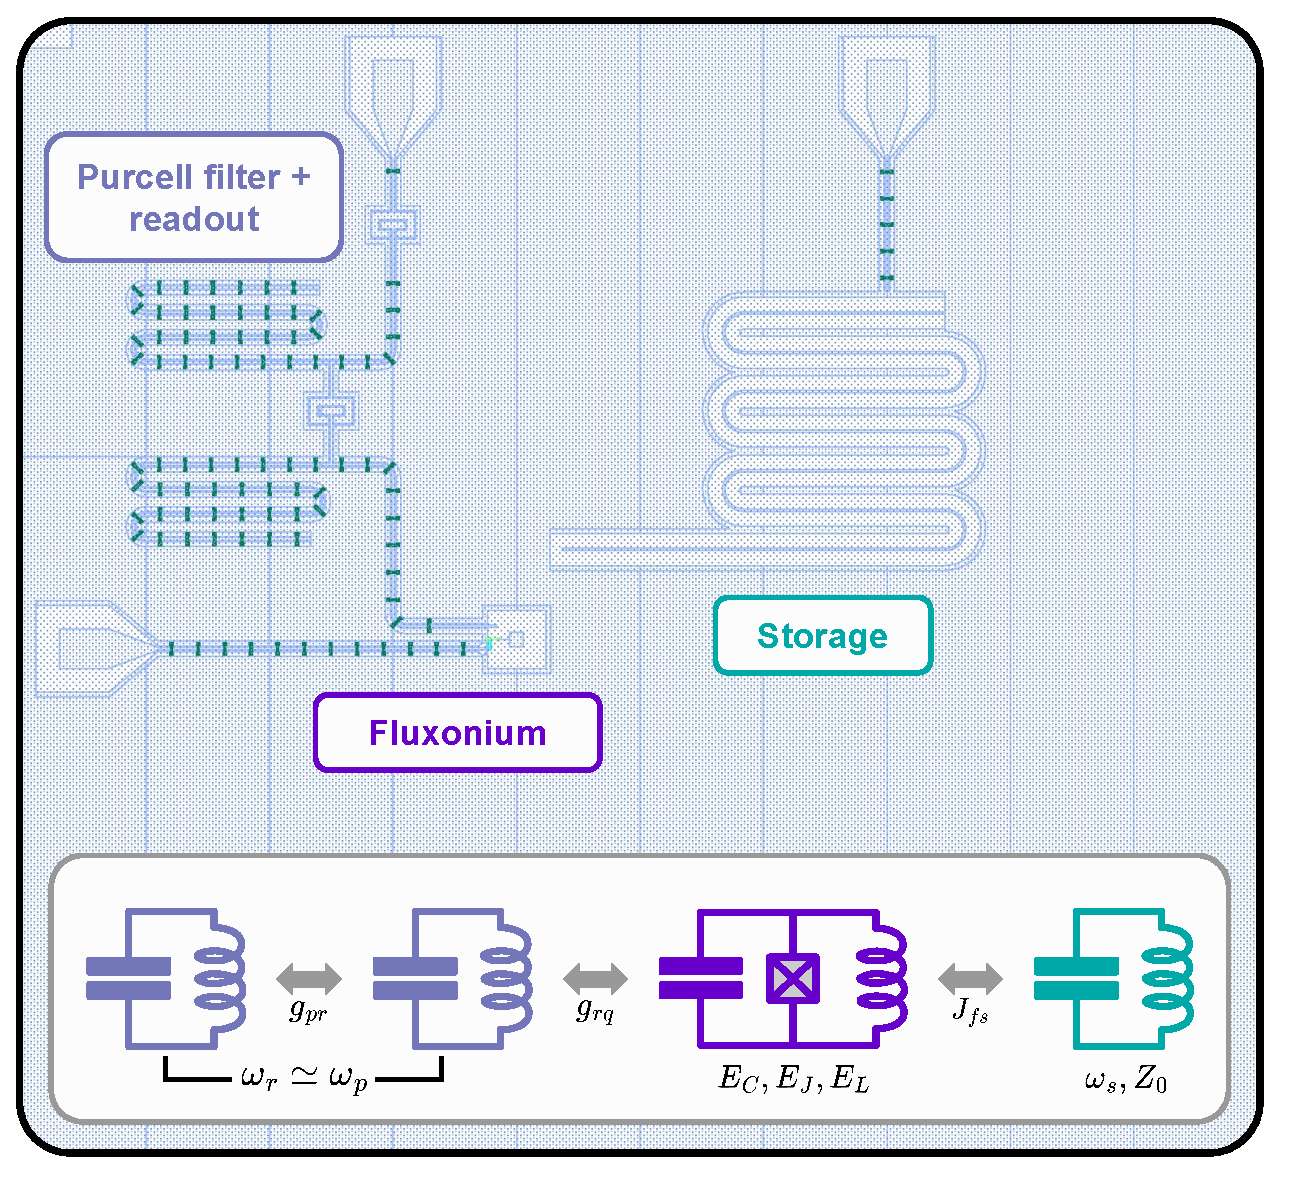
\includegraphics[width=0.8\linewidth]{Figures/5/2D_Dispersive_GDS.pdf}
        \vspace*{2mm}
    \end{subfigure} 
    \begin{subfigure}{\linewidth}
        \centering
        \begin{tabular}{c|c|c|c|c|c|c|c|c }
       $\omega_s/2\pi$ & $J_{fs}/2\pi$ & $E_J/h$  & $E_C/h$ & $E_L/h$ & $g_{rq}/2\pi$ & $\omega_r/2\pi$ & $\omega_p/2\pi$ & $g_{pr}/2\pi$\\\hline
        4134.0 & 3.0 & 3754.9 & 844.0 & 299.9 & 42.1 & 6125.0 & 6137.0 & 27.6
    \end{tabular}
    \end{subfigure}
    \caption{Final GDS design and parameters for the 2D dispersive experiment, showing the on-chip storage resonator, fluxonium qubit, readout resonator, and Purcell filter. The frequency parameters for the various elements in the table are all listed in MHz}
    \label{fig:5_2D_Dispersive_GDS}
\end{figure}

\noindent \textbf{Fluxonium:} We chose the nominal qubit parameters $E_J, E_C, E_L$ shown above in Fig. \ref{fig:5_2D_Dispersive_GDS} to achieve a moderately heavy fluxonium with a frequency of $\omega_q/2\pi \simeq 107$ MHz at half-flux. We expect this will result in a long $T_1^{g\to e}$ away from the sweet spot. These parameters also ensured that the qubit plasmon transition frequencies were high enough to not be limited by heating out of the $\ket{g}$-$\ket{e}$ manifold. 


\noindent \textbf{Storage and Fluxonium System:} The storage mode was designed as a large gap (60 $\mu$m) $\lambda/4$ coplanar waveguide resonator with a resulting impedance of $Z_0 = 95.127$ $\Omega$. We chose its frequency to be as low as possible to maximize $T_1$ given a constant $Q = \omega_s T_1$, ultimately settling on $\omega_s/2\pi = 4.134$ GHz. This was co-designed with the fluxonium so as to achieve bosonic mode threading. For the fluxonium-storage coupling $J_{fs}$, we performed numerical diagonalization simulations of the following Hamiltonian (similar to that in Ch. \ref{sec:4_3D_Experiment_Design_Theory}):
\begin{equation}
    \hat{H} =  \hat{H}_s + \hat{H}_{\rm int} + \hat{H}_{\rm fluxonium} =  \omega_s \hat{a}^\dagger \hat{a} + J_{fs} \hat{n}\hat{n}_a + \Big[4E_C \hat{n}^2 + \frac{1}{2}\hat{\varphi}^2 - E_J\cos(\hat{\varphi}-\varphi_{\rm ext})\Big],
\end{equation}
using which we calculated the dispersive shift $\chi = \omega_s^{|e\rangle} - \omega_s^{|g\rangle} = [E_{e,1} - E_{e, 0}] - [E_{g, 1} - E_{g, 0}]$ as well as the storage Kerr nonlinearities $K = (K_g + K_e)/2$ and $dK = (K_g - K_e)/2$ defined by $K_{g/e} = E_{g/e, 2} + E_{g/e, 0} - 2E_{g/e, 1}$. We then manually varied $\omega_s$ and $J_{fs}$ so as to achieve a low $K$ and $dK$ (on the order of Hz)\footnote{We have seen in simulations that the average Kerr $K$ is worse for GKP performance than differential Kerr $dK$. We can typically afford $dK$ to be slightly (as much as 5-10x) larger than $K$; ideally we have $K < 5$ Hz.} over the external flux range of interest $\Phi_{\rm ext}/\Phi_0 \in [0.43, 0.5]$, while also having a flux-tunable $\chi$ that crosses through zero and that is large enough away from this zero-crossing to perform ECD. We tried to target similar values for $\chi$, $K$, and $dK$ as Ref. \cite{sivak2023gkp-expt}, and ultimately picked a flux operating point with $\chi/2\pi \simeq 50$ kHz, $K/2\pi \simeq 1$ Hz, and $dK/2\pi \simeq 10$ Hz, as shown in Fig. \ref{fig:5_2D_disp_chi_and_Kerr} 
\begin{figure}[h]
    \centering
    % \includegraphics{}
    \caption{\todo{make this figure!}}
    \label{fig:5_2D_disp_chi_and_Kerr}
\end{figure}

\noindent \textbf{Readout and Purcell Filter:} We used a similar design for the readout resonator and Purcell filter as the RAF; both resonators were standard 50 $\Omega$ coplanar waveguide resonators with frequencies $\omega_r/2\pi = 6.125$ and $\omega_p/2\pi = 6.137$. We chose $g_{pr}$ to be greater than the detuning of the modes, so that the two are almost fully hybridized with normal mode frequencies of roughly $\omega_r - g_{pr}$ and $\omega_p + g_{pr}$ [to see this, diagonalize $\hat{H}_{pr} = \omega_r\hat{r}^\dagger \hat{r} + \omega_p\hat{p}^\dagger \hat{p} + g_{pr}(\hat{r}^\dagger\hat{p} + \hat{r}\hat{p}^\dagger)$]. The Purcell filter is strongly coupled to a transmission line with a coupling of $\kappa_p/2\pi \simeq 38.8$ MHz and, choosing $g_{pr} \lesssim \kappa_p$, results in an effective linewidth of the readout of $\kappa_r/2\pi \simeq 16$ MHz. 


identical nominal frequencies of $\omega_r/2\pi = 6.125$ GHz. The two resonators are coupled via the Hamiltonian
\begin{equation}
    \hat{H}_{pr} = \omega_r\hat{r}^\dagger \hat{r} + \omega_p\hat{p}^\dagger \hat{p} + g_{pr}(\hat{r}-\hat{r}^\dagger)(\hat{p} - \hat{p}^\dagger)
\end{equation}
from which we get normal modes with frequencies $\approx \omega_r \pm g_{pr}$ for the hybridized system. The Purcell filter is strongly coupled to a transmission line with a coupling of $\kappa_p/2\pi \simeq 38.8$ MHz. We chose 


As further shown in Fig. \ref{fig:5_SBS_Sideband_Reset}, our proposed approach to implement the qubit reset here is to use direct fluxonium sideband cooling by driving the $\ket{e0}\leftrightarrow\ket{g1}$ transition between the qubit and readout resonator. 


\subsection{Performance Estimates}

The first check we carried out when assessing the feasibility of a 2D dispersive design was to determine how quickly we can implement a round of SBS (i.e. one quadrature of QEC). We based this on preliminary simulations from our theory collaborators Jonathan Pelletier and Baptiste Royer that indicated\footnote{These simulations aren't yet published, but they show that the maximum storage photon number at which ECD starts to break in simulation is similar or even slightly higher for a fluxonium than for a transmon.} that a fluxonium qubit is not significantly different than a transmon from the perspective of carrying out ECD. As a result (cf. above), we designed our storage-fluxonium system to have a similar dispersive shift and Kerr nonlinearity as the storage-transmon system from Ref. \cite{sivak2023gkp-expt}, and assumed in what follows that we can use a similar photon number (approximately 100-140 storage photons) in ECD. 
\begin{figure}[h]
    \centering
 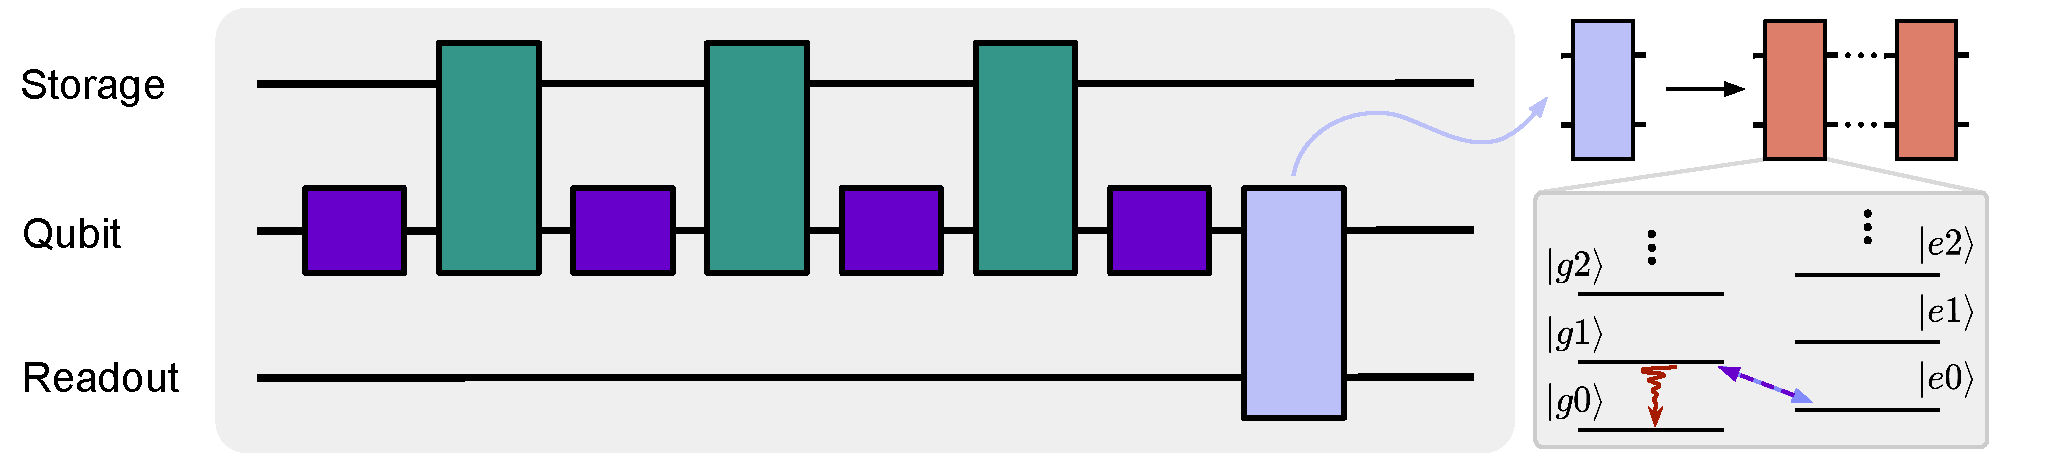
\includegraphics[width=\linewidth]{Figures/5/SBS_Sideband_Reset.pdf}
    \caption{SBS sequence consisting of 3 conditional displacements (teal), 4 qubit pulses (purple),  and unconditional qubit reset (lilac). The reset can be further decomposed into a number of dissipative swap operations based on fluxonium $\ket{e0}\leftrightarrow\ket{g1}$ sideband cooling.}
    \label{fig:5_SBS_Sideband_Reset}
\end{figure}

\noindent The sequence for SBS is shown in Fig. \ref{fig:5_SBS_Sideband_Reset}: it consists of 4 conditional displacements (CDs), 3 qubit $\pi/2$ rotations, and qubit reset. We assume our CDs take the same time as Ref. \cite{sivak2023gkp-expt} and that our qubit pulses each take 32 ns; meanwhile for reset, we follow Ref. \cite{nordquantique2023gkp-expt} where the authors used $N_{\rm reset} = 2$ dissipative swaps. In our case, our readout has a linewidth of $\kappa_r / 2\pi \approx 9$ MHz, giving a $T_1 \simeq 18$ ns. We thus take $T_{\rm diss. swap} \simeq 132$ ns (which is $\sim\!6T_1$ plus some buffer). In total, the time $\delta t$ that we estimate it will take for a round of SBS is:
\begin{align*}
\delta t = T_{\rm sBs}  &= 4T_{\rm pi} + (T_{\rm CD\,1} + T_{\rm CD\,2} + T_{\rm CD\,3}) + \big[N_{\text{reset}}\times T_{\text{diss. swap}}\big] \\ &= 4\times (32) + (470 + 676 + 230) + \Big[2 \times 132\Big] = 1768\, {\rm ns}
\end{align*}